\documentclass[aspectratio=169,11pt]{beamer}
% ==========================================================================
%  KSA lecture-slide theme  =  stock beamer "Boadilla"  +  KSA colour theme
%  brand colours sampled from the official KSA symbol mark:
%    Deep Prussian Blue  #2E3192   (지성 - intellect)
%    Golden Gray         #D6CBB1   (감성 - sensibility)
%  Engine: XeLaTeX.  Usage:
%    \documentclass[aspectratio=169,11pt]{beamer}
%    \input{../../theme/ksa-theme.tex}
%  Each deck lives in its own slides/kor/<deck>/ folder together with its
%  own images; ../../figs/ is kept only as a fallback for the shared cache.
% ==========================================================================

\usepackage{fontspec}
\usepackage{amsmath,amssymb}
\usepackage{graphicx}
\graphicspath{{figs/}{./}{../../../figs/}}
\usepackage{booktabs}
\usepackage{listings}
\usepackage{varwidth}

% ---- fonts (no ctex/xeCJK on this box -> fontspec drives CJK directly) -----
\defaultfontfeatures{Ligatures=TeX}
\setmainfont{Noto Sans CJK KR}
\setsansfont{Noto Sans CJK KR}
\setmonofont{Noto Sans Mono CJK KR}[Scale=0.92]

% ---- base theme: stock Boadilla ------------------------------------------
\usetheme{Boadilla}
\usefonttheme{professionalfonts}
\setbeamertemplate{navigation symbols}{}

% ---- KSA colour theme (recolour the stock theme) --------------------------
\definecolor{ksablue}{HTML}{2E3192}
\definecolor{ksabluedk}{HTML}{20226A}
\definecolor{ksagold}{HTML}{D6CBB1}
\definecolor{ksagolddk}{HTML}{A9976B}
\definecolor{ksared}{HTML}{C0392B}
\definecolor{ksagray}{HTML}{5B5B5B}

\setbeamercolor{structure}{fg=ksablue}
\setbeamercolor{alerted text}{fg=ksared}

\setbeamercolor{palette primary}{fg=white,           bg=ksablue}
\setbeamercolor{palette secondary}{fg=white,         bg=ksablue!85!black}
\setbeamercolor{palette tertiary}{fg=white,          bg=ksabluedk}
\setbeamercolor{titlelike}{fg=ksablue}
\setbeamercolor{frametitle}{fg=ksablue,bg=}
\setbeamercolor{title}{fg=ksablue}
\setbeamercolor{author}{fg=ksagray}
\setbeamercolor{institute}{fg=ksagray}
\setbeamercolor{block title}{fg=white,bg=ksablue}
\setbeamercolor{block body}{fg=black!85,bg=ksablue!6}
\setbeamercolor{item}{fg=ksablue}
\setbeamercolor{section in toc}{fg=black!85}

\setbeamerfont{frametitle}{series=\bfseries}
\setbeamerfont{title}{series=\bfseries}

% ---- footline:  KSA mark | "Made by ..." | n / N   (matches reference) ----
\newcommand{\ksacredit}{}
\setbeamertemplate{footline}{%
  \hbox{%
    \begin{beamercolorbox}[wd=.18\paperwidth,ht=2.6ex,dp=1.5ex,leftskip=1.1em]{}%
      \raisebox{-0.35ex}{\includegraphics[height=2.0ex]{ksa-logo.png}}%
    \end{beamercolorbox}%
    \begin{beamercolorbox}[wd=.64\paperwidth,ht=2.6ex,dp=1.5ex,center]{}%
      {\scriptsize\color{ksagray}\ksacredit}%
    \end{beamercolorbox}%
    \begin{beamercolorbox}[wd=.18\paperwidth,ht=2.6ex,dp=1.5ex,rightskip=1.1em]{}%
      \hfill{\scriptsize\color{ksablue}\insertframenumber\,/\,\inserttotalframenumber}%
    \end{beamercolorbox}%
  }%
  \vskip2pt
}

% ---- section divider: stock \sectionpage, KSA-coloured -------------------
\setbeamertemplate{section page}{%
  \begingroup\centering
    {\color{ksagolddk}\rule{0.16\paperwidth}{1pt}}\par\vskip1.0em
    {\usebeamerfont{title}\color{ksablue}\insertsectionhead\par}\vskip1.0em
    {\color{ksagolddk}\rule{0.16\paperwidth}{1pt}}\par
  \endgroup
}
\AtBeginSection[]{\begin{frame}[plain,noframenumbering]\vfill\sectionpage\vfill\end{frame}}

% ---- code listings ------------------------------------------------------------
\lstdefinestyle{ksa}{%
  basicstyle=\ttfamily\scriptsize,
  keywordstyle=\color{ksablue}\bfseries,
  commentstyle=\color{ksagray}\itshape,
  stringstyle=\color{ksagolddk},
  numberstyle=\tiny\color{ksagray},
  backgroundcolor=\color{ksablue!6},
  frame=leftline, framerule=1.4pt, rulecolor=\color{ksablue},
  xleftmargin=1em, aboveskip=0.8em, belowskip=0.4em,
  showstringspaces=false, breaklines=true, language=Python,
}
\lstset{style=ksa}

% ---- handy macros -----------------------------------------------------------
\newcommand{\kb}[1]{\textbf{\color{ksablue}#1}}   % blue keyword
\newcommand{\kq}[1]{\textbf{\color{ksared}#1}}    % red key-question

\setbeamerfont{title}{series=\bfseries,size=\fontsize{24}{30}\selectfont}
\setbeamerfont{subtitle}{series=\bfseries,size=\fontsize{14}{18}\selectfont}
\setbeamerfont{author}{size=\normalsize}
\setbeamerfont{institute}{size=\small}
\graphicspath{{figs/}{../../../../assets/}}
\makeatletter
\newcommand{\markpage}[1]{\protected@write\@auxout{}{\string\newlabel{#1}{{\the\c@framenumber}{}}}\hypertarget{#1}{}}
\newcommand{\pref}[1]{\hyperlink{#1}{\textcolor{ksagolddk}{(p.\ref{#1})}}}
\makeatother

\renewcommand{\ksacredit}{Machine Learning 1 \,\textperiodcentered\, Seq2Seq}
\title{Seq2Seq 시퀀스투시퀀스 (Sequence to Sequence)}
\subtitle{읽는 신경망 하나, 쓰는 신경망 하나}
\author{Machine Learning 1}
\institute{한국과학영재학교 (KSA)}
\date{}
\begin{document}
\begin{frame}[plain,noframenumbering]\titlepage\end{frame}


% --- 오늘의 질문
\begin{frame}{오늘의 질문: 길이가 다른 문장을 어떻게 번역할까?}
\vfill
\centering
{\Huge I \quad love \quad you \quad $\longrightarrow$ \quad \textcolor{ksared}{Je \quad t'aime}}\vskip1em
{\large 영어 \kb{3}단어 $\to$ 프랑스어 \kq{2}단어 \quad 순서도 다르다 (te = you 가 동사 앞)}\\[0.8em]
{\large 지난 시간의 RNN: 한 칸 읽을 때마다 한 칸 내놓는다 \quad $\Rightarrow$ 입력과 출력의 길이가 같아야}
\vfill
\note{I love you, 영어 세 단어가 프랑스어로는 Je t'aime 두 단어입니다. 길이도 다르고, 순서도 다릅니다. you에 해당하는 te가 동사 앞에 옵니다. 지난 시간의 RNN 글자 모델은 한 칸 읽을 때마다 한 칸을 내놓았습니다. 그러면 입력과 출력의 길이가 같아야 하고, 순서도 맞아야 합니다. 번역은 이 틀에 맞지 않습니다. 오늘은 이 문제를 푼 Seq2Seq를 배웁니다.}
\end{frame}

% --- 아이디어
\begin{frame}{Seq2Seq: 다 읽고 나서 쓴다}
\markpage{idea}
\vfill
\centering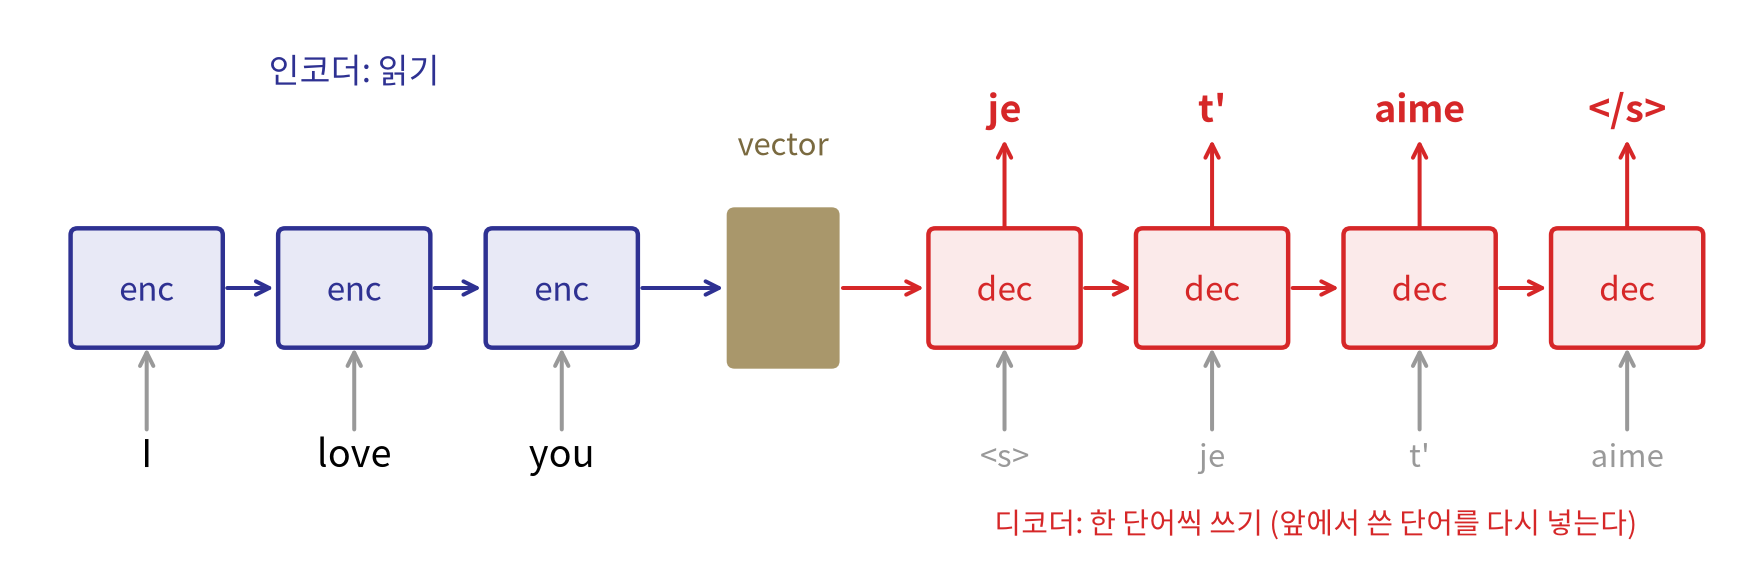
\includegraphics[width=0.88\linewidth]{s2s_encdec.png}\par\vskip0.2em
{\large \textcolor{ksablue}{인코더} RNN 이 문장을 \textbf{벡터 하나}로 \quad $\to$ \quad \textcolor{ksared}{디코더} RNN 이 단어를 하나씩}\\[0.1em]{\large \texttt{</s>} (끝) 가 나오면 멈춘다 \quad 그래서 길이가 달라도 된다}\\[0.2em]
{\small Sutskever, Vinyals, Le (Google, 2014) \quad 같은 해 Cho 외 (GRU 를 제안한 논문) 도 같은 구조}
\vfill
\note{Seq2Seq, 시퀀스 투 시퀀스는 2014년 구글의 수츠케버, 비냘스, 레가 발표했습니다. 아이디어는 간단합니다. 먼저 인코더 RNN이 문장을 끝까지 다 읽고, 마지막 메모, 즉 벡터 하나에 문장 전체를 담습니다. 그다음 디코더 RNN이 그 벡터에서 출발해 단어를 하나씩 씁니다. 디코더는 앞에서 쓴 단어를 다시 입력으로 받아 다음 단어를 정하고, 끝 표시가 나오면 멈춥니다. 그래서 입력과 출력의 길이가 달라도 됩니다. 같은 해 GRU를 제안한 조경현 교수 팀의 논문도 같은 구조를 썼습니다.}
\end{frame}

% --- 식
\begin{frame}{식으로}
\vfill
\centering
\renewcommand{\arraystretch}{1.6}
{\Large\begin{tabular}{rl}
\textcolor{ksablue}{인코더} & $\mathbf{h}_t = \text{RNN}_{\text{enc}}(\mathbf{h}_{t-1}, \mathbf{x}_t), \quad \mathbf{v} = \mathbf{h}_T$\\
\textcolor{ksared}{디코더} & $\mathbf{s}_0 = \mathbf{v}, \quad \mathbf{s}_k = \text{RNN}_{\text{dec}}(\mathbf{s}_{k-1}, y_{k-1})$\\
다음 단어 & $P(y_k \mid y_{<k}, \mathbf{x}) = \text{softmax}(W \mathbf{s}_k)$
\end{tabular}}\vskip0.6em
{\LARGE\[ P(\mathbf{y} \mid \mathbf{x}) = \prod_{k} P(y_k \mid y_{<k}, \mathbf{x}) \]}\vskip0.2em
{\large 손실 = 정답 단어마다 $-\log P$ 를 더한 것 (교차 엔트로피)}\\[0.2em]{\large 입력 문장이 통째로 \textbf{벡터 $\mathbf{v}$ 하나}를 지나간다}
\vfill
\note{식으로 쓰면, 인코더는 지난 시간의 RNN 그대로 입력 단어 x를 하나씩 읽어 메모 h를 고쳐 쓰고, 마지막 메모를 벡터 v라 합니다. 디코더는 v에서 출발해, 앞에서 쓴 단어 y를 넣어 메모 s를 고쳐 쓰고, s에 행렬을 곱해 softmax로 다음 단어의 확률을 냅니다. 문장 전체의 확률은 단어별 확률의 곱이고, 학습은 정답 단어마다 마이너스 로그 확률을 더한 교차 엔트로피를 줄이는 겁니다. 중요한 건 입력 문장의 모든 정보가 벡터 v 하나를 지나가야 한다는 점입니다.}
\end{frame}

% --- 학습 vs 사용
\begin{frame}{배울 때와 쓸 때}
\vfill
\centering
\renewcommand{\arraystretch}{1.6}
{\large\begin{tabular}{lll}
 & 디코더에 넣는 앞 단어 & \\\hline
배울 때 & \textbf{정답} 단어 (\texttt{<s>}, je, t') & teacher forcing: 한 번에 모든 칸을 계산\\
쓸 때 & \textbf{자기가 쓴} 단어 & 한 단어씩, 가장 확률 높은 단어를 고른다 (greedy)
\end{tabular}}\vskip0.8em
{\large 논문: 후보 문장 몇 개를 함께 이어 가는 \textbf{빔 서치} (beam search) \quad 후보 2개로도 충분}\\[0.4em]
{\small 첫 단어를 틀리면 다음 단어도 틀리기 쉽다: 틀린 단어가 다시 입력으로 들어가니까}
\vfill
\note{배울 때와 쓸 때가 조금 다릅니다. 배울 때는 디코더에 정답 단어를 넣어 줍니다. 시작 표시, je, t'를 넣고 각각 다음 단어 je, t', aime를 맞히게 하죠. 이걸 선생님이 정답을 알려 준다고 해서 teacher forcing이라 하고, 모든 칸을 한 번에 계산할 수 있습니다. 쓸 때는 정답이 없으니 자기가 쓴 단어를 다음 입력으로 넣습니다. 가장 확률 높은 단어를 고르는 방법이 greedy이고, 논문은 후보 문장 몇 개를 동시에 이어 가는 빔 서치를 썼습니다. 빔 크기 2로도 충분했다고 합니다. 첫 단어를 틀리면 그 단어가 다시 들어가 다음 단어도 틀리기 쉽다는 점도 기억해 두세요.}
\end{frame}

% --- 실험 A
\begin{frame}{실험: 영어 숫자 말 $\to$ 숫자}
\markpage{expA}
\vfill
\centering
{\large 0 $\sim$ 999 를 영어로 쓴 말 $\to$ 숫자 \quad 800개로 배우고, 본 적 없는 200개로 시험}\vskip0.6em
\renewcommand{\arraystretch}{1.3}
\begin{tabular}{lcc}
입력 (단어 1 $\sim$ 4개) & 출력 (글자 1 $\sim$ 3개) & \\\hline
six hundred ninety six & 696 & \textcolor{ksablue}{O}\\
eight hundred one & 801 & \textcolor{ksablue}{O}\\
forty six & 46 & \textcolor{ksablue}{O}\\\hline
nine hundred fifty two & 952 & \textcolor{ksablue}{O}\\\hline
seventy & \textcolor{ksared}{77} & 정답 70
\end{tabular}\vskip0.6em
{\large 시험 정답률 \kb{99.5\%} (200개 중 199개) \quad 틀린 1개: \textbf{0 이 말에 없는} seventy}
\vfill
\note{작은 실험을 해 봤습니다. 0부터 999까지를 영어로 쓴 말, 예를 들어 six hundred ninety six를 숫자 696으로 바꾸는 번역입니다. 입력은 단어 1개에서 4개, 출력은 글자 1개에서 3개로 길이가 다릅니다. 1000개 중 800개로 배우고, 본 적 없는 200개로 시험했더니 199개, 99.5퍼센트를 맞혔습니다. 틀린 하나가 재밌습니다. seventy를 77로 썼습니다. 70의 0은 말로 나타나지 않으니, 디코더가 두 번째 글자를 쓸 때 벡터에서 일의 자리가 없다는 걸 읽어 내야 하는데, seventy seven 같은 말과 헷갈린 겁니다.}
\end{frame}

% --- 논문 결과
\begin{frame}{논문: 영어 $\to$ 프랑스어 (WMT'14)}
\vfill
\centering
\renewcommand{\arraystretch}{1.5}
{\large\begin{tabular}{ll}
모델 & LSTM \textbf{4층} × 1,000칸 \quad 문장 하나 = 숫자 \kb{8,000}개 (4층 × $\mathbf{h}$, $\mathbf{c}$ × 1,000)\\
데이터 & 문장 쌍 1,200만 개\\
결과 & BLEU \kb{34.8} (LSTM 5개 앙상블) \quad vs \quad 기존 통계 번역 33.3
\end{tabular}}\vskip0.8em
{\large 신경망만으로 큰 번역 대회에서 기존 방법을 \textbf{처음} 넘었다}\\[0.4em]
{\small BLEU: 기계 번역이 사람 번역과 단어 묶음 (1 $\sim$ 4단어) 이 얼마나 겹치는지 0 $\sim$ 100 점}
\vfill
\note{논문의 실제 번역 실험입니다. LSTM 4층에 층마다 1000칸을 써서, 문장 하나를 숫자 8000개로 표현했습니다. 층마다 h와 c가 1000칸씩이니 4 곱하기 2 곱하기 1000입니다. 문장 쌍 1200만 개로 학습해, LSTM 5개를 합친 앙상블이 BLEU 34.8점을 받아 기존 통계 번역 33.3점을 넘었습니다. 신경망만으로 큰 번역 대회에서 기존 방법을 처음 넘은 결과입니다. BLEU는 기계 번역이 사람 번역과 단어 묶음이 얼마나 겹치는지를 0에서 100점으로 잰 점수입니다.}
\end{frame}

% --- 거꾸로
\begin{frame}{요령: 입력을 거꾸로 넣기}
\markpage{reverse}
\vfill
\centering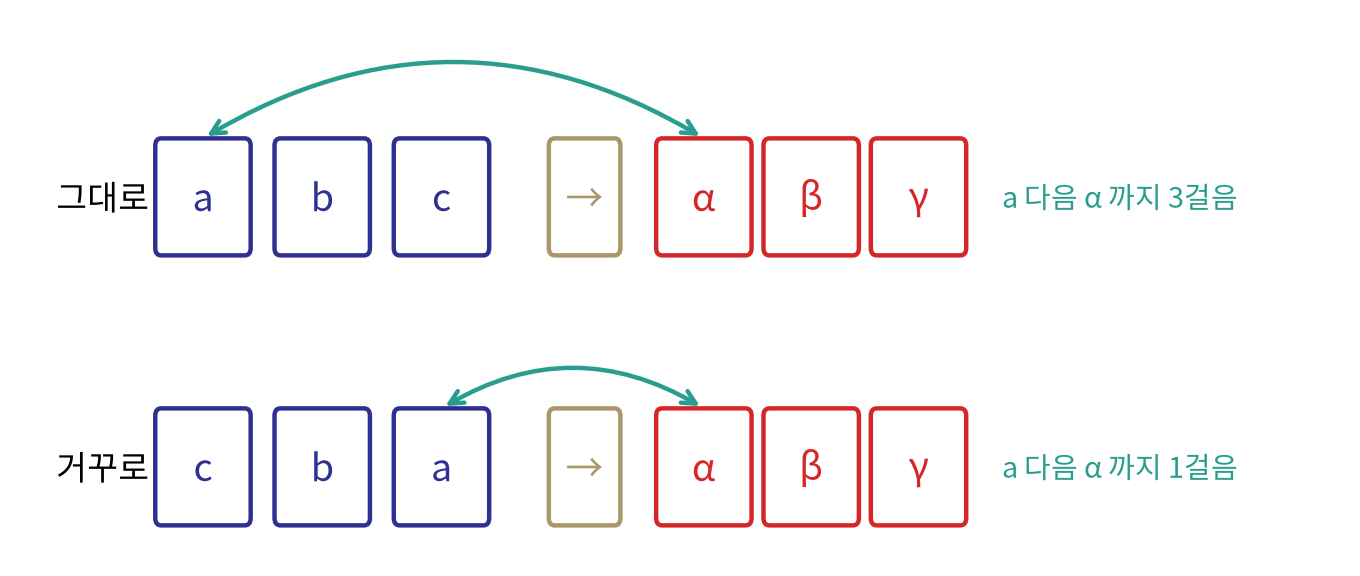
\includegraphics[width=0.62\linewidth]{s2s_reverse.png}\par\vskip0.2em
{\large 입력 단어 순서만 뒤집었더니 BLEU \kq{25.9} $\to$ \kb{30.6}}\\[0.3em]
{\large 첫 단어끼리 가까워져 \textbf{연결을 배우기 쉬워진다}}\\[0.2em]{\small 뒤 단어끼리는 멀어져서 평균 거리는 같다}
\vfill
\note{논문의 재밌는 요령입니다. 입력 문장의 단어 순서만 뒤집어 넣었더니 BLEU가 25.9에서 30.6으로 올랐습니다. 그대로 넣으면 첫 단어 a를 읽고 b, c를 지나 3걸음 뒤에야 α를 씁니다. 거꾸로 넣으면 a를 마지막에 읽으니 바로 다음 걸음에 α를 씁니다. 대응하는 단어끼리 평균 거리는 같지만, 첫 단어끼리 가까워지면 학습 초기에 연결을 잡기 쉬워지고, 첫 단어를 맞히면 그다음도 잘 풀린다고 논문은 설명합니다.}
\end{frame}

% --- 실험 B
\begin{frame}{실험: 벡터 하나는 비좁다}
\markpage{expB}
\vfill
\centering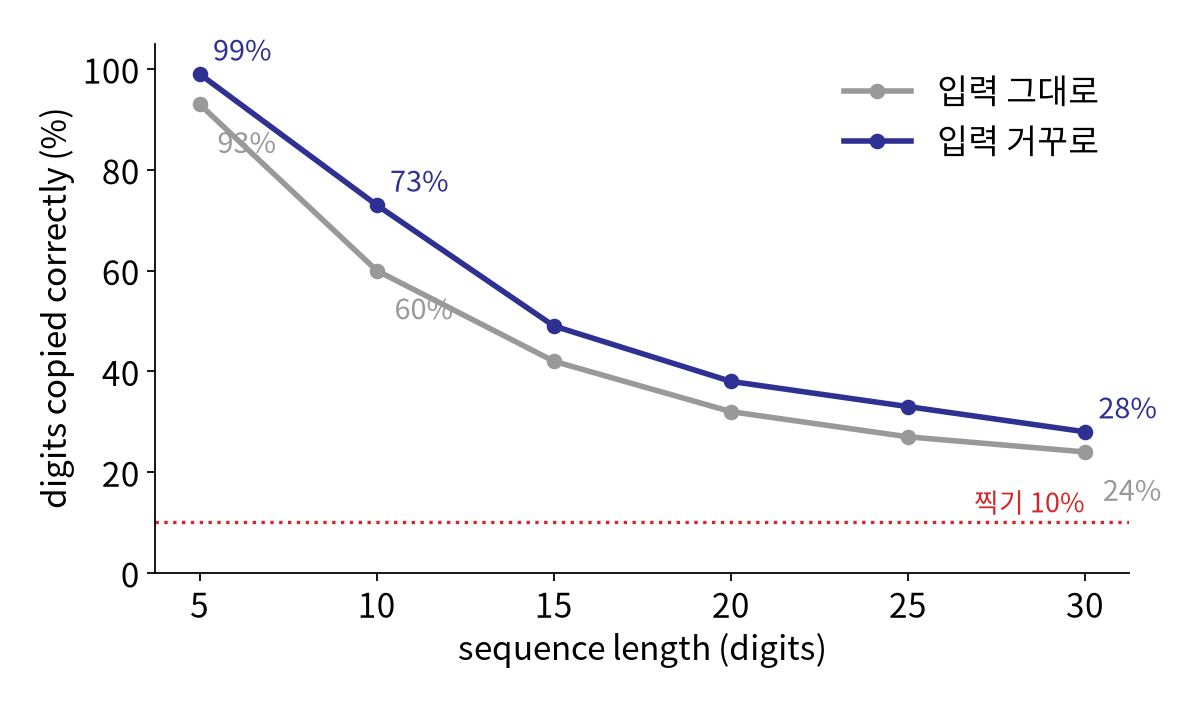
\includegraphics[width=0.56\linewidth]{s2s_copy.png}\par\vskip0.2em
{\large 숫자열을 \textbf{그대로 베끼기} \quad 벡터 32칸 (GRU) \quad 길이 5: \kb{93\%} $\to$ 길이 30: \kq{24\%}}\\[0.2em]
{\large 통째로 맞힌 비율: 길이 5 에서 89\% (거꾸로 99\%), 길이 20 부터 0\%}
\vfill
\note{두 번째 실험은 가장 쉬운 번역, 숫자열을 그대로 베끼기입니다. 벡터 32칸짜리 GRU로, 길이 5부터 30까지 섞어 학습했습니다. 길이 5에서는 숫자의 93퍼센트를 맞히지만, 길이가 늘수록 떨어져 30에서는 24퍼센트, 찍기 10퍼센트에 가까워집니다. 숫자열 전체를 통째로 맞힌 비율은 길이 5에서 89퍼센트, 20부터는 0입니다. 정보가 아무리 많아도 벡터 32칸 하나를 지나가야 하니까요. 파란 선처럼 거꾸로 넣으면 조금 낫지만, 병목 자체를 없애지는 못합니다.}
\end{frame}

% --- 한계 → 어텐션
\begin{frame}{한계와 다음 걸음: 어텐션}
\vfill
\centering
{\large 문장이 길수록 벡터 하나에 다 담기 어렵다 \quad (논문은 거꾸로 넣기 덕에 긴 문장도 버텼다)}\vskip0.8em
\renewcommand{\arraystretch}{1.6}
{\large\begin{tabular}{ll}
Seq2Seq & 디코더는 \textbf{마지막} 벡터 $\mathbf{v}$ 하나만 본다\\
\textbf{어텐션} & 단어를 쓸 때마다 인코더의 \kb{모든 칸} $\mathbf{h}_1, \dots, \mathbf{h}_T$ 를 다시 본다
\end{tabular}}\vskip0.8em
{\large ``je'' 를 쓸 때는 I 를, ``aime'' 를 쓸 때는 love 를 주로 본다 \quad $\to$ 다음 시간}\\[0.3em]{\small 어텐션: Bahdanau, Cho, Bengio (2014)}
\vfill
\note{정리하면 Seq2Seq의 한계는 문장이 길수록 벡터 하나에 다 담기 어렵다는 겁니다. 논문은 거꾸로 넣기 같은 요령으로 버텼죠. 같은 해 바다나우, 조경현, 벤지오는 다른 방법을 냈습니다. 디코더가 마지막 벡터 하나만 보지 말고, 단어를 쓸 때마다 인코더의 모든 칸을 다시 보자는 겁니다. je를 쓸 때는 I를, aime를 쓸 때는 love를 주로 보는 식이죠. 이게 어텐션이고, 다음 시간에 배웁니다.}
\end{frame}

% --- 문제풀이
\begin{frame}{문제풀이}
\vfill
\begin{enumerate}
\item 디코더가 세 단어에 확률 0.5, 0.8, 0.9 를 주고 \texttt{</s>} 에 0.5 를 주었다. 문장 전체의 확률과 손실 ($-\ln$) 은?\vskip0.8em
\item 입력 a b c d 를 그대로 / 거꾸로 넣을 때, a 를 읽은 뒤 α 를 쓰기까지 각각 몇 걸음?\vskip0.8em
\item 디코더가 \texttt{</s>} 를 내놓지 못하면 어떻게 될까? 실제로는 어떻게 막을까?\vskip0.8em
\item 실험 A 에서 ``seventy'' $\to$ 77 처럼 틀린 이유를, 출력 길이와 벡터의 관점에서 설명해 보라.
\end{enumerate}
\vfill
\note{1번 답. 0.5 곱하기 0.8 곱하기 0.9 곱하기 0.5, 0.18이고, 손실은 마이너스 ln 0.18, 약 1.71입니다. 2번 답. 그대로면 a를 읽고 b, c, d를 지나 4걸음, 거꾸로면 1걸음입니다. 3번 답. 끝없이 단어를 씁니다. 그래서 최대 길이를 정해 두고 거기서 멈춥니다. 4번 답. 70은 seventy 한 단어인데 출력은 두 글자이고, 0은 입력에 없습니다. 디코더가 두 번째 글자를 쓸 때 벡터에서 일의 자리를 읽어야 하는데, 7이 들어간 다른 말들처럼 7을 써 버린 겁니다.}
\end{frame}

% --- 실습
\begin{frame}{실습}
\vfill
\centering\begin{tabular}{rl}
\large 1 & 영어 숫자 말 만들기 \texttt{words(904)} $\to$ nine hundred four, 데이터 준비\\[0.5em]
\large 2 & GRU 인코더-디코더 학습 (teacher forcing) $\to$ greedy 로 번역, 틀린 예 보기\\[0.5em]
\large 3 & 숫자열 베끼기: 길이별 정답률, 입력 그대로 vs 거꾸로
\end{tabular}\vskip1em
\href{https://colab.research.google.com/github/SuminHan/book-ml/blob/main/slides/v2/ml1/week12/seq2seq/lab/seq2seq.ipynb}{\textcolor{ksagolddk}{▶ Colab에서 실습 노트북 열기}}
\vfill
\note{실습은 세 부분입니다. 첫째, 숫자를 영어 말로 바꾸는 함수를 만들어 데이터를 준비합니다. 둘째, GRU 인코더-디코더를 teacher forcing으로 학습하고 greedy로 번역해 틀린 예를 봅니다. 셋째, 숫자열 베끼기로 길이별 정답률을 재고 입력을 거꾸로 넣으면 어떻게 달라지는지 확인합니다.}
\end{frame}

% --- 정리
\begin{frame}{정리}
\vfill
\centering\large\begin{tabular}{l}
\textbf{Seq2Seq}: 인코더가 문장을 \kb{벡터 하나}로, 디코더가 한 단어씩 \texttt{</s>} 까지\\[0.5em]
배울 때는 정답 단어를 (teacher forcing), 쓸 때는 자기가 쓴 단어를 넣는다\\[0.5em]
2014 영어 $\to$ 프랑스어 BLEU 34.8 > 통계 번역 33.3 \quad 거꾸로 넣기 25.9 $\to$ 30.6\\[0.5em]
한계: 벡터 하나는 비좁다 (베끼기 93\% $\to$ 24\%) \quad 다음: 어텐션
\end{tabular}
\vfill
\note{정리합니다. Seq2Seq는 인코더가 문장을 벡터 하나로 담고, 디코더가 그 벡터에서 단어를 하나씩 끝 표시까지 써서, 입력과 출력의 길이가 달라도 됩니다. 배울 때는 정답 단어를, 쓸 때는 자기가 쓴 단어를 넣습니다. 2014년 영어 프랑스어 번역에서 BLEU 34.8로 통계 번역을 처음 넘었고, 입력을 거꾸로 넣는 요령으로 25.9에서 30.6이 되었습니다. 한계는 벡터 하나가 비좁다는 것, 베끼기 실험에서 길이 5는 93퍼센트지만 30은 24퍼센트였습니다. 다음 시간에는 이 한계를 푼 어텐션을 배웁니다.}
\end{frame}
\end{document}
